\documentclass{article}
\usepackage[utf8]{inputenc}
\usepackage{amsmath}%AMS Math Package Importing

\title{Period 6 LaTeX Example}
\author{Ishaan Sathaye }
\date{October 13 2020}

\usepackage{natbib}
\usepackage{graphicx}

\begin{document}%all code will be below this

\maketitle %makes the preamble shown, which is above this code

\section{Introduction}%making a new section
This is the first section. In LaTeX, new lines are manual.It will wrap text automatically but not make new line breaks.\\ 
This is a new line.

%Math
Inline math doesn't separate the math from the sentence. Like $f(x)=x^25$\\
Display math is centered and on it's own line. $$\int_2^3{f(x)dx}$$ like that.
To make matrices:
$$
\begin{matrix}
2 & 3 & 4 \\
a & b & c
\end{matrix}
$$
$$
\begin{bmatrix}
2 & 3 & 4 \\
a & b & c
\end{bmatrix}
$$
$$
\begin{vmatrix}
2 & 3 & 4 \\
a & b & c
\end{vmatrix}
$$
Fraction is $$\frac{4}{5}$$

There is a theory which states that if ever anyone discovers exactly what the Universe is for and why it is here, it will instantly disappear and be replaced by something even more bizarre and inexplicable.
There is another theory which states that this has already happened.

\begin{figure}[h!]
\centering
%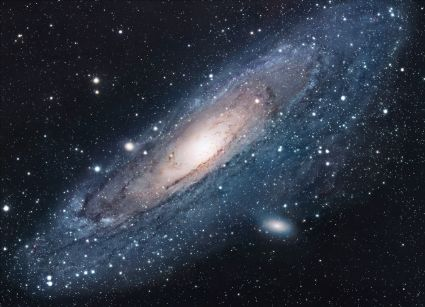
\includegraphics[scale=1.7]{universe}
\caption{The Universe}
\label{fig:universe}
\end{figure}

\section{Conclusion}
%``I always thought something was fundamentally wrong with the universe'' \citep{adams1995hitchhiker}

\section{Final Thoughts}

\bibliographystyle{plain}
\bibliography{references}
\end{document}
